\section{Conceptos Previos}

\begin{frame}{Modelica} 
    \begin{itemize}
        \item Lenguaje de modelado orientado a objetos.
        \item Modelado de sistemas complejos, con componentes mecánicos, eléctricos, electrónicos, hidráulicos, térmicos, etc.     
        \item Desarrollado por la asociación sin fines de lucro ``Modelica Asociation''.        
        \item Los modelo son descriptos en texto plano.        
        \item Entornos de desarrollo: OpenModelica, MathModelica, Dymola, etc.
        \item Librería con componentes ya definidos.
    \end{itemize}
\end{frame}
 

\begin{frame}[fragile]
\frametitle{Clases} 
\begin{columns}  
\column{.5\textwidth}  
\begin{block}{}
\begin{itemize}
    \item Define un objeto.
    \item Son instanciadas mediante la definición de variables.
    \item Tienen tres secciones:
        \begin{enumerate}
            \item Definiciones.
            \item Ecuaciones.
            \item Sentencias.
        \end{enumerate}
    \item Clases especializadas:  \textit{model}, \textit{record}, \textit{block}, \textit{connector}, \textit{function}, \textit{package}   
\end{itemize}
\end{block}{}
\column{.5\textwidth}
\begin{lstlisting}[style=base]
    class X
        // Definiciones de 
                variables y clases   
    equation
        // Ecuaciones
    statements
        // Sentencias
    end X;   
\end{lstlisting}
\end{columns}
\end{frame}

%\begin{frame}[fragile]
%\frametitle{Prefijos de Clases} 
%Prefijos de clase: \textit{model}, \textit{record}, \textit{block}, \textit{connector}, \textit{function}, \textit{package}
%\begin{itemize}
%    \item Mejoran la lectura del código:
%    \item Agregan restricciones a la clase
%\end{itemize}   
%
%\begin{columns}  
%\column{.5\textwidth}  
%\begin{lstlisting}[style=base]
%    class Circuits
%        cclass Pin
%            Real v;
%            flow Real i;
%        end Pin;
%        class Componente
%            Pin n,p;
%        equation 
%            n.v = p.v;
%        end Componente; 
%    end Circuits;   
%\end{lstlisting}
%\par
%\column{.5\textwidth}
%\begin{lstlisting}[style=base]
%    @package@ Circuits
%        @connector@ Pin
%            Real v;
%            flow Real i;
%        end Pin;
%        @model@ Componente
%            Pin n,p;
%        equation 
%            n.v = p.v;
%        end Componente; 
%    end Circuits;   
%\end{lstlisting}
%\par
%\end{columns}
%\end{frame}





\begin{frame}[fragile]
\frametitle{Herencias de Clases} 
\begin{columns}  
\column[t]{8cm}  

\begin{block}{}
\begin{itemize}
    \item Agrega significado semántico al modelo.
    \item Facilita la reutilización de código.
    \item Se utiliza la palabra reservada: \textit{extends}.
\end{itemize} 
\end{block}

\begin{block}{}
La clase hijo obtiene las características del padre.
\end{block}

\column[t]{5cm}  
\begin{lstlisting}[style=base]
model OnePort
    Pin p;
    Pin n;
    Real v;
    Real i;
equation
    v = p.v - n.v;
    i = p.i;
    i = -n.i;
end OnePort;
model Capacitor
    @extends@ OnePort;
    parameter Real C = 1;
equation
    C * der(v) = i;
end Capacitor;
\end{lstlisting}
\end{columns}
\end{frame}

\begin{frame}[fragile]
\frametitle{Tipos de Variables} 
\begin{columns}  
\column[t]{9cm}
\begin{block}{}
    \begin{itemize}
        \item \textbf{Tipos básicos}: \textit{Real}, \textit{Integer}, \textit{Boolean}.
        \item Las clases definen un nuevo tipo.
        \item \textbf{Sinónimos de tipos}.
        \item \textbf{Prefijos de Tipo}: \textit{flow}, \textit{constant}, \textit{parameter}, \textit{discrete}, \textit{input} y \textit{output}.
    \end{itemize} 
\end{block}
\column[t]{5cm}
\begin{lstlisting}[style=base]
    type Current = flow Real;
    type Voltage = Real;
    connector Pin
        Voltage v;
        Current i;
    end Pin;
    
    type TenPin = Pin[10];
    
    TenPin pines;
    Pin pines2 [10];
\end{lstlisting}
\par
\end{columns}
\end{frame}


\begin{frame}[fragile]
\frametitle{Modificaciones} 
\begin{columns}  
\column[T]{7cm}
\begin{block}{Aparecen en}
\begin{enumerate}
    \item Declaraciones de variables.
    \item Sinónimo de tipo.
    \item Definiciones de herencia.
\end{enumerate} 
\end{block}

\begin{block}{Podemos}
\begin{enumerate}
    \item Cambiar el valor inicial de una variable.    
    \item Redefinir una variable.
    \item Cambiar la definición de un tipo.
    \item Anidar modificaciones.
\end{enumerate}
\end{block}
\column[T]{7cm}
\begin{lstlisting}[style=base]
package Circuits
    model CircuitX
        Capacitor cap;
        Resistor res;
        ...
    equation 
    
    ...
        
    end CircuitX;
    model MainCircuit
        Capacitor x(C = 2);
        CircuitX co1 (cap(C = 10));
        CircuitX co2 (cap(C = 15));
    end MainCircuit;
end Circuits;
\end{lstlisting}

 
\end{columns}
\end{frame}

\begin{frame}[fragile,t]
\frametitle{Ecuaciones} 
\begin{block}{}
Las ecuaciones no representan una asignación, sino igualdades.\\ Pueden tener expresiones complejas de ambos lados de la igualdad y expresan una relación entre las variables.
\end{block}
\vspace{0.1cm}
\begin{columns}  
\column[t]{4cm}
Ecuaciones de Igualdad
\vspace{0.2cm}
\begin{lstlisting}[style=base]
p.v - n.v = v;

p.v - n.v -v = 0;

p.v - v = n.v ;

\end{lstlisting} 
\column[t]{5cm}
\pause
Ecuación \textit{for}
\vspace{0.2cm}
\begin{lstlisting}[style=base]
for i in 1:N loop
    v[i] = p[i].v - n[i].v; 
end for;
\end{lstlisting} 
\column[t]{4cm} 
\pause
N = 4
\vspace{0.2cm}
\begin{lstlisting}[style=base]
v[1] = p[1].v - n[1].v;       
v[2] = p[2].v - n[2].v;
v[3] = p[3].v - n[3].v;
v[4] = p[4].v - n[4].v;
\end{lstlisting} 
\end{columns}
\end{frame}

\begin{frame}[fragile]
\frametitle{Ecuaciones \textit{connect}} 
\begin{block}{Conectores}
\begin{itemize}
\item Son clases con ciertas restricciones.
\item Se definen con el prefijo \textit{connector}.
\item No tienen ecuaciones.
\item Tienen dos categorías de variables:
    \begin{itemize}
        \item Variables de potencial. Ejemplo: presión, voltaje, etc. 
        \item Variables de flujo: definidas con el prefijo flow. Ejemplo: corriente, caudal, etc.
    \end{itemize} 
\end{itemize}
\end{block}
\begin{block}{Ejemplo}
Clase Pin:
\begin{itemize}
    \item Voltaje: Variables de potencial.
    \item Corriente: Variables de flujo.
\end{itemize}
\end{block}
\end{frame}

\begin{frame}[fragile]
\frametitle{Ecuaciones \textit{connect}} 
\begin{block}{Ecuaciones \textit{connect}}
    \begin{itemize}
        \item Conectan dos clases del mismo tipo.
        \item Genera relaciones entre las variables internas de los conectores:
            \begin{itemize}
                \item Las variables de potencial dentro de una misma conexión deben ser iguales entre sí.
                \item Las variables de flujo siguen las reglas de Kirchhoff: la suma de los flujos es igual a cero. 
        \end{itemize}
    \end{itemize}
\end{block}{}
\pause
\begin{columns}  
\column[T]{8cm}
 \begin{lstlisting}[style=base,,basicstyle=\scriptsize]
    model LC_circuit
        Capacitor cap(v(start = 1));
        inductor ind(L = 2);
        ground gr;
    equation
        connect(ind.p,cap.p);
        @connect(ind.n,cap.n);@
        @connect(cap.n,gr.p);@
    end LC_circuit;
\end{lstlisting}
\column[T]{6cm}
 \begin{lstlisting}[style=base]
    // Variables de Potencial 
    ind.n.v  = cap.n.v;
    cap.n.v = gr.p.v;
    
    // Variables de flujo 
    ind.n.i + cap.n.i + gr.p.i = 0;
\end{lstlisting}
% Mencionar que se tiene que resolver a nivel global las conexiones
\end{columns}
\end{frame}

\begin{frame}[fragile]
\frametitle{Modelo aplanado} 
\begin{block}{Modelo aplanado}
\begin{enumerate}
\item Modelo monolítico.
\item No tiene clases.
\item Variables de tipo básicos.
\item No posee ecuaciones \textit{connect}.
\end{enumerate}
\end{block}
\end{frame}

\begin{frame}[fragile]
\frametitle{Tama\~nos de un modelo} 
\begin{block}{Tamaño de la descripción}
Consideramos la cantidad de clases, variables, ecuaciones, etc. definidas.
\end{block}
\begin{block}{Tamaño del sistema}
Consideramos la dimensionalidad del modelo. Cantidad total de variables. 
\end{block}
\pause
\begin{block}{}
\begin{lstlisting}[style=base,,basicstyle=\scriptsize]
model Big
    parameter Integer N = 1000000;
    Real a[N];
equation
    for i in 1:N loop
        a[i] = i * 10;
    end for;
end Big;
\end{lstlisting}
\end{block}
\end{frame}

%% antes mencionar que trabajamos con modelos con arreglos y ecuaciones for
%% Cambiar grafico por Parsing -> Flattering -> Index Reduction -> 
%% Se hace muy grande el modelo si expandimos
\begin{frame}[fragile]
\frametitle{Simulación de Modelos Modelica} 
    \begin{figure}
      \centering
      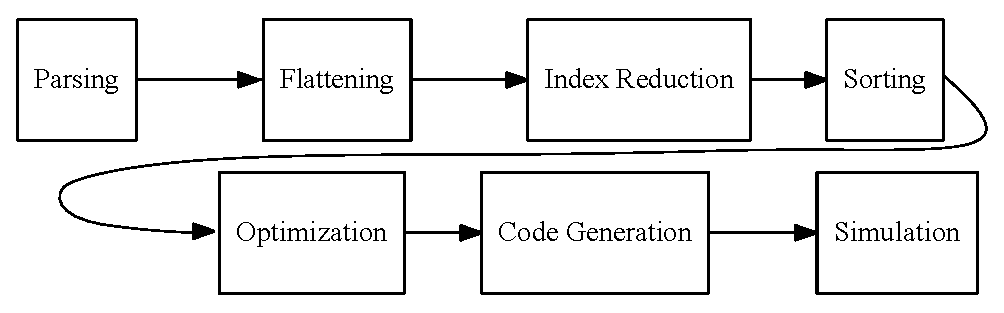
\includegraphics[scale=0.8]{pipeline} 
      \label{fig:proceso}
    \end{figure}
\end{frame}



\begin{frame}[fragile]
\frametitle{Simulación de Modelos Grandes} 
\begin{block}{Problemas}
Expandir las variables y ecuaciones vectorizadas implica un alto costo computacional en las siguientes etapas de compilación. \\
Imposibilidad de trabajar con sistemas de grandes dimensiones.
\end{block} 
\pause
\begin{block}{Objetivos}
Algoritmo de aplanado con costo computacional constante con respecto a la dimensionalidad (cantidad de variables) del modelo. \\
Mantener las definiciones de arreglos y ecuaciones \textit{for} durante toda la etapa de compilación.
\end{block} 
\end{frame}
